\documentclass[oneside]{nccuthesis}
\usepackage{times}
\usepackage{verbatim}
\usepackage{color}
\usepackage{url}
\usepackage{graphicx}
\usepackage{array}
\usepackage{pdfpages} % include outside .pdf
\usepackage{wallpaper} % watermark
% for table generate
\usepackage{mathtools}
\usepackage{amsmath}
\usepackage{amssymb}
\usepackage{booktabs}
\usepackage{adjustbox}

\usepackage{amsmath,amssymb,amsfonts,amsthm}
\usepackage[normalem]{ulem}
\usepackage{graphicx}
\usepackage{textcomp}
\usepackage{xcolor}
\usepackage{tikz}
\usepackage{algorithm}
\usepackage[algo2e]{algorithm2e}
\usepackage{algcompatible}
\usepackage{algpseudocode}
\usepackage{amsfonts}
\usepackage{amssymb}
\usepackage{amsmath}
\usepackage{amsthm}
\usepackage{url}
\usepackage{indentfirst}
\usepackage{multirow}
\usepackage{mathtools}
%
\usepackage{graphicx}
\usepackage{titlesec}
\usepackage{titletoc}
\usepackage{CJKnumb}
 \titleformat{\chapter}{\centering\Huge\bfseries}{第\,\CJKnumber{\thechapter}\,章}{1em} {}


\newtheorem{definition}{Definition}
\newtheorem{theorem}{Theorem}
\newtheorem{lemma}{Lemma}
\newtheorem{game}{Game}\setcounter{game}{-1}
\newtheorem{game1}{Game}[game]
\newtheorem{claim}{Claim}

% Format the refs
\usepackage[square,sort,comma,numbers]{natbib}
\usepackage[hidelinks]{hyperref}

% For the tree
\usepackage{tikz}
\usepackage{tikz-qtree}

% For barchart
\usepackage{pgfplots}

% Using the tex-text mapping for ligatures etc.
\defaultfontfeatures{Mapping=tex-text}

% Set the default fonts
\setmainfont{Times New Roman}
\setCJKmainfont{標楷體}

% Your information goes here
% author: Tz-Huan Huang [http://www.csie.ntu.edu.tw/~tzhuan]

% ----------------------------------------------------------------------------
% "THE CHOCOLATE-WARE LICENSE":
% Tz-Huan Huang wrote this file. As long as you retain this notice you
% can do whatever you want with this stuff. If we meet some day, and you think
% this stuff is worth it, you can buy me a chocolate in return Tz-Huan Huang
% ----------------------------------------------------------------------------

% Syntax: \var{English}{Chinese}
\university{National Chengchi University}{國立政治大學}
\college{College of Science}{理學院}
\institute{Department of Computer Science}{資訊科學系}
\title{A Simple Two-Step Byzantine Fault Tolerance in Private Blockchains}{私有區塊鏈上的兩步驟拜占庭共識演算法}
\author{Jian-Wei Su}{蘇鑑微 \ }
\studentid{106753006}
\advisor{Tung-Wei Kuo, Ph.D.}{郭桐惟 \ 博士}
\defenseyear{2019}{一零八}
\defensemonth{September}{九}
\defenseday{15}

\pgfplotsset{compat=1.14}
\begin{document}

% 政大論文浮水印
% 政大論文浮水印
% \CenterWallPaper{0.174}{pdfs/watermark.pdf}
% \setlength{\wpXoffset}{6.1725cm}
% \setlength{\wpYoffset}{10.5225cm}

\CenterWallPaper{}{pdfs/watermark.pdf}
\setlength{\wpXoffset}{0pt}
\setlength{\wpYoffset}{0pt}

\hypersetup{pageanchor=false}

\frontmatter
\pagenumbering{gobble}
\makecover

\clearpages
\setcounter{page}{1}
\hypersetup{pageanchor=true}
\pagenumbering{roman}
\phantomsection

% generate certification
% \makecertification
% or include scanned pdf
\addcontentsline{toc}{chapter}{口試委員會審定書}
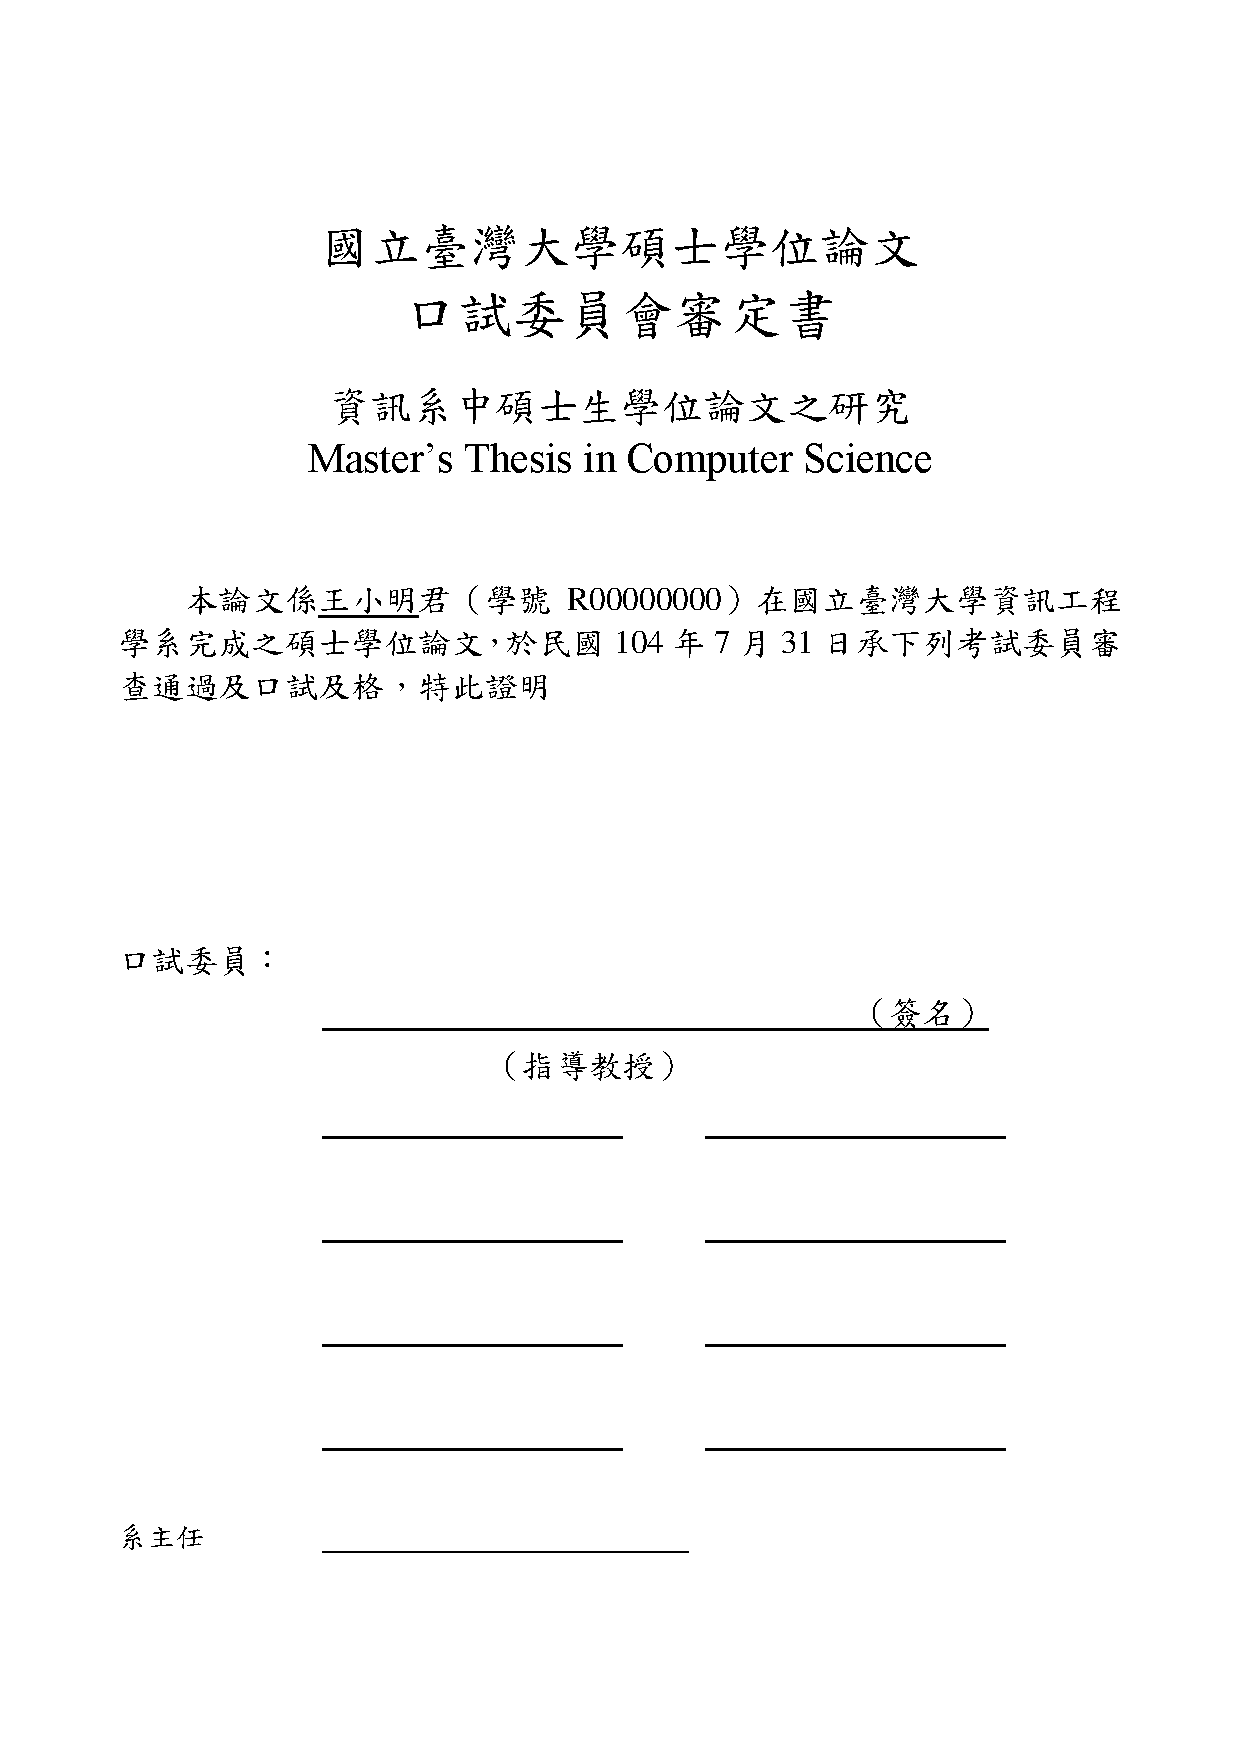
\includepdf[pages={1}]{pdfs/cert.pdf}

%\begin{acknowledgementszh}
首先要誠摯的感謝指導教授郭桐惟老師兩年多來的照顧、指導與鼓勵,不論是學業或是研究方向,都給予了我很大的幫助,使我能順利地完成論文撰寫,圓滿完成碩士研究。在此也要感謝口式委員XXX及XXX,抽空審閱與指導此篇論文,並提出寶貴的意見,因為有你們,這篇論文才可以更加完整。\\

同時也要感謝實驗室的同學,仁傑,子源,勤文,禾暘等幾位同學與學長姐,因為有你們的互相幫忙,提供協助與諮詢,我才能順利完成研究。\\

最後我要感謝我的家人,在我念研究所時,不離不棄,成為我永源最健強的後盾,沒有你們就沒有今天的我。

感謝\ldots
\end{acknowledgementszh}



\begin{abstractzh}
區塊鏈技術至今已發展十多年歷程。區塊鏈應用也從一開始數位貨  幣衍伸生出多樣化的應用與服務。區塊鏈是一種分散式帳本技術,帳本內容是由多個網路節點共同維護,而非受到單一節點所控制。為了確保安全性,系統內所有節點,需要擁有相同帳本資料;換句話說,節點間須對帳本內容達成共識,而達成共識的方法稱共識演算法。為因應不同的應用情境,區塊鏈分為公有鏈與私有鏈。公有鏈對所有人皆開放,而私有鏈只開放特定人群或企業加入。本篇論文針對私有鏈上的共識演算法進行探討及研究。一般而言,私有鏈共識演算法需要三個步驟的訊息交流,才能確保共識結果是正確的。我們設計了一個兩步驟的共識演算法-TwoStep­BFT。此演算法能夠容許拜占庭節點錯誤,且保有安全性及活性。為了架設大規模節點的私有鏈,我們整合了多樣的自動化雲端部屬套件,此套件幫助我們在雲端平台上自動產生節點並分析共識結果。實驗結果顯示我們的方法在一百個節點依舊能有300TPS的共識效率。

\noindent
關鍵字: 區塊鏈、共識演算法、拜占庭容錯。 
\end{abstractzh}

\begin{abstracten}
Blockchain technologies have been developed for more than ten years. Deriving from digital currency, blockchains also expands diversified applications and services. Blockchains can be divided into public chains and private chains. The public chains are open to everyone, and the private chains are only open to specific groups or companies. The key property of blockchains is decentralization, meaning that content is not generated by specific nodes but created by multiple nodes in the system. We need a consensus algorithm to make the blockchains consistent. This paper explore the consensus algorithm on the private chains. Generally speaking, the consensus algorithm usually requires three steps of information exchange to ensure that the consensus result is exact. We designed a two steps consensus algorithm, TwoStepBFT, which allows the Byzantine attack and maintains safety. In order to experiment in several nodes, we integrated a variety of automated tools to deploy private blockchains and analyze experimental results on the cloud platform. Experimental results have shown that our consensus still has 300 TPS on one hundred nodes. \\
	
\noindent
Keywords: Blockchain, Consensus Algorithm, Byzantine Fault Tolerance, Automation. 
\end{abstracten}


% Table of Content
\clearpages
\tableofcontents
% List of Figures
\if0
\clearpages
\listoffigures
\fi
% List of Tables
%\clearpages
%\listoftables

\mainmatter

% Your thesis goes here
\chapter{緒論}
從1969年網際網路誕生以來,眾多數位化的商品與服務不斷推陳出新,進而大幅改變了人們的生活習慣。然而,貨幣的數位化卻是直到近年來區塊鏈的誕生才得以真正的被實現。良好的數位貨幣系統需要具備下列三特性:
(一)交易紀錄難以被竄改、(二)避免雙花(Double-spending)、(三)避免由某個單一角色控制該數位貨幣系統,下列分別介紹此三項特性。

(一) 交易紀錄難以被竄改:交易紀錄與網路訊息一樣,只是單純的位元碼。如何確定使用者擁有某數位貨幣資產,並保證交易紀錄無法遭人輕易竄改,是非常重要的問題。

(二)避免雙花:在數位貨幣系統中,可能存在同一筆數位資產,因為不當操作而被重複使用的情況,這類問題也被稱之為「雙花問題」。

(三)避免由某個單一角色控制該數位貨幣系統:如果系統中存有一個中央集權的角色,例如:中央政府或金融企業等,來協助交易的清算及交易記錄的保存,那麼前兩項特性是容易被滿足的。這類做法雖然頗具效率,但是賦予單一集權角色過大權力卻可能導致不好的結果。例如:國家能夠透過加印鈔票來稀釋鈔票的價值,進而控制金融市場;遊戲公司也可能透過發行新的虛擬點數,讓原先的虛擬點數一文不值。

區塊鏈便是能同時滿足難以被竄改、無法重複支付且去除中央集權的安全系統。區塊鏈是一種基於分散式系統(Distributed system)的節點備份技術,系統中每一位參與者為稱之為節點。節點間權力相互平等,不需透過中央集權角色來管理系統運作。每一個節點都各自擁有一份帳本資料,節點間會相互溝通合作,來確保所有節點的帳本資料是一致的。因此,攻擊者難以透過攻擊單一節點來癱瘓整個系統運作。在區塊鏈系統裡,所有節點所看到的帳本內容是相同的,帳本內交易順序相同,如此一來節點就能根據帳本內的交易順序了解交易是否生效。
區塊鏈是由連續的區塊所組成,區塊內記錄了節點們所提交的交易內容。區塊之間通過保存哈希值(Hash)實現鏈接。為了增加惡意攻擊難度,區塊內會包含該區塊產生的時間戳(Timestamp)。為了防止惡意節點任意更動過去的帳本資料,每一個區塊會包含一個獨一無二的哈希值,該值是根據前一個區塊的內容所產生的。惡意攻擊者無法任意更動前面的區塊內容。一旦區塊內容改變,哈希值將無法符合,這樣的設計使得區塊鏈變得更加安全。第一個區塊稱為創世區塊(Genesis block),創世區塊是所有區塊中,唯一不需要包含前一個區塊哈希值的特例區塊。
\begin{figure}[!htbp]
\centering
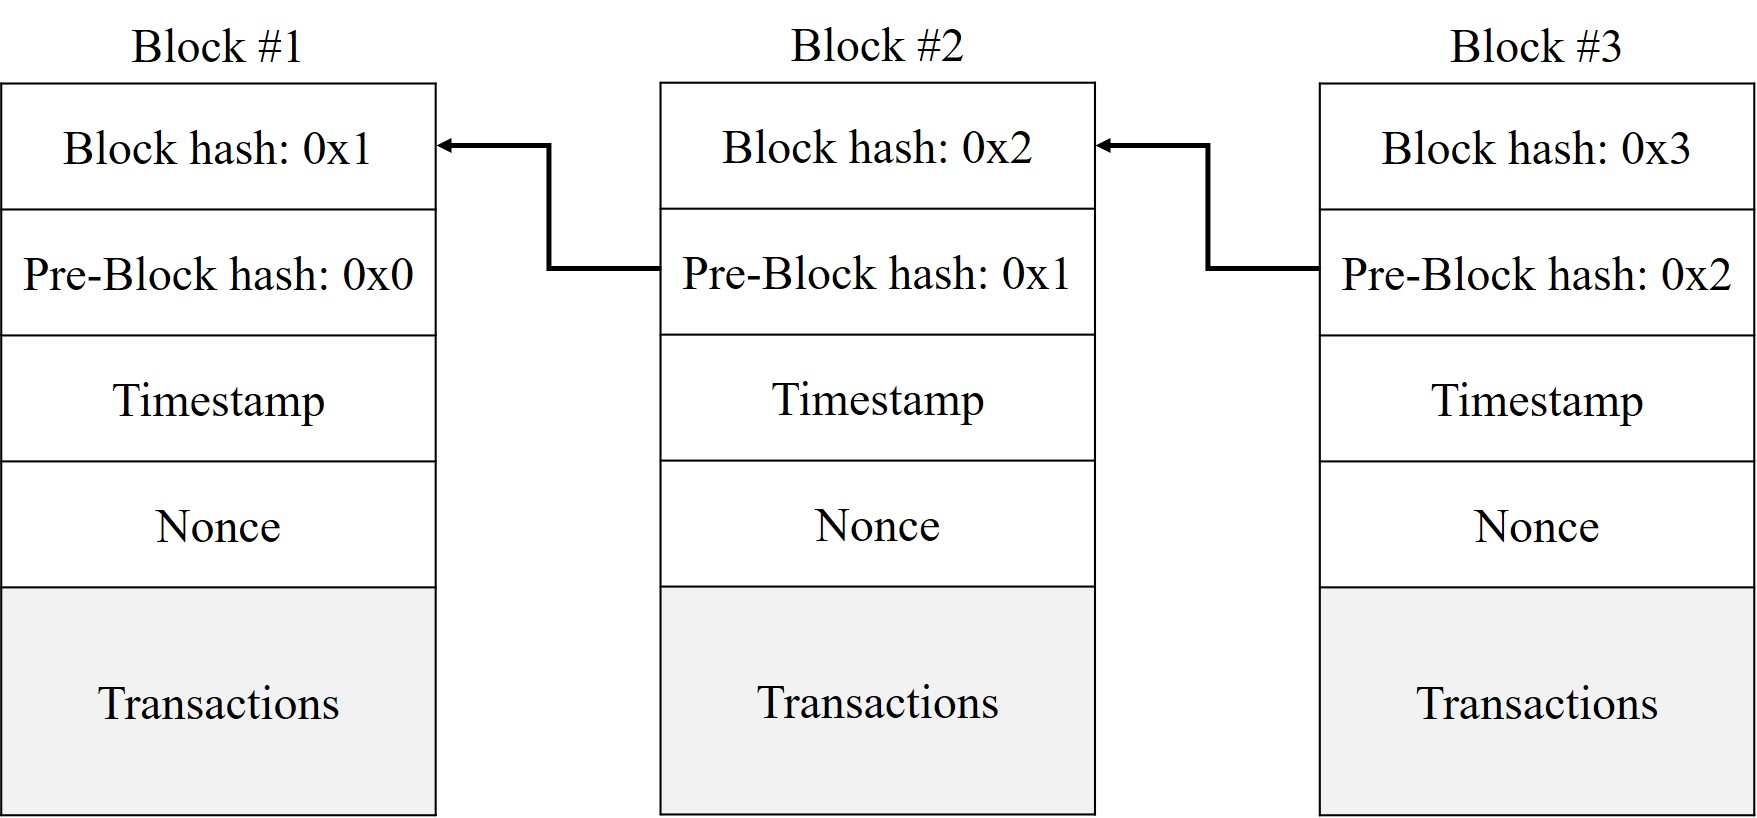
\includegraphics[scale=0.5]{images/1.jpg}
\caption{區塊鏈示意圖}
\label{i:byz-latency}
\end{figure}


因應不同用戶需求及應用場景,區塊鏈系統架構及規模也不盡相同。區塊鏈主要類型可分為公有鏈以及私有鏈。公有鏈的應用如比特幣 \cite{Bitcoin}或以太幣 \cite{Ethereum}等,其特性為任何人都能參與該區塊鏈,加入公有鏈不需要任何人授權,可以隨時自由加入或退出。不同於公有鏈,私有鏈大多是指多個機構共同參與管理的區塊鏈,每個機構執行一個或多個節點,參與私有鏈的節點須有嚴格規範。私有鏈上知名例子包含Facebook Libra \cite{STEVE_HANNA2010}、R3 Corda \cite{R3}等。私有鏈中的資料只允許系統內不同的機構進行讀寫,並且共同記錄及備份資料。由於參與私有鏈的節點是有限制和可控制的,因此私有鏈往往可以有較快的交易速度、更好的隱私保護且不容易被惡意攻擊。本論文將聚焦於私有鏈上。
因為區塊鏈是一個分散式架構,節點間平權管理,所以需要透過運行相同的「共識協議」來維護相同的區塊順序。這類的共識協議則稱為共識演算法。公有鏈上的共識演算法大多採工作量證明(PoW)來達成共識。PoW(Proof-of-Work)透過競賽解題,第一個解出題目的節點將獲得廣播區塊的權力,共識過程中大部分的運算效能都會花在這個解題步驟(俗稱挖礦),因此區塊產出時間會被拉長,導致共識效率低落。然而私有鏈因為節點需經授權才可加入,這類演算法大多透過投票來選擇區塊的廣播者,透過輪流廣播來維持區塊鏈內的平權治理。

私有鏈上通常運行BFT共識演算法,BFT是拜占庭容錯(Byzantine Fault-Tolerant)的縮寫。在拜占庭容錯的區塊鏈上,即使系統中部分節點當機或存在惡意節點情況下,區塊鏈依舊具備安全性(Safety)與活性(Liveness)等性質。安全性能夠保證區塊鏈上每個參與區塊鏈系統的節點,都擁有相同且排序一致的帳本內容。活性則讓區塊鏈是一個永續的系統,能夠容忍錯誤發生且避免因為單一節點故障而導致系統停擺。目前已經有許多BFT共識演算法,傳統的BFT演算法通常需要多個回合才能達成共識。每一個回合會有一個節點擔任提議者(Proposer)。一般來說,一個回合需要執行三個步驟:第一個步驟的目的在於讓提議者廣播其提議,若該提議者廣播多份提議,則區塊鏈可能發生分叉(Fork)進而導致內容衝突。這讓攻擊者可能重複花費同一筆金錢;第二個步驟的目的即為讓所有節點檢查該提議者是否只有廣播一份提議。若提議者只有廣播一份提議,在第三個步驟中,節點便可以開始投票(將收到的提議廣播給其他節點),若一個節點蒐集到足夠多的同意票,該節點便可以確認該提議為最終共識結果;第三個步驟的目的是為了克服訊息傳輸延遲,知名的BFT演算法PBFT \cite{castro1999practical}便是根據上述三個步驟設計。

過去也有少部分的BFT演算法在一個回合中只需要兩個步驟,例子包含FaB \cite{abraham2018revisiting}、Zyzzyva \cite{kotla2007zyzzyva}、SBFT \cite{martin2006fast}、Hydrachain \cite{Hydrachain}。然而,FaB與Zyzzyva已被指出無法保證活性,換句話說,共識演算法可能永遠無法達成共識。另一方面,Hydrachain也被指出無法保證安全性,也就是說,不同的正常節點可能會有不同的共識節果,這在區塊鏈上及代表分岔。雖然SBFT能夠保證安全性與活性,但是SBFT在節點發生故障或是網路延遲過大的情況下,會改用類似PBFT的三步驟設計。因此,在系統狀況良好時,SBFT每回合只需要執行兩個步驟。但是在系統狀況不良時,SBFT每回合仍需要執行三個步驟。
本論文探討的議題為一個新的兩回合拜占庭共識演算法。更明確的說我們希望在不犧牲安全性及活性情況下,設計一個每回合只需要兩個步驟的BFT演算法。重要的是,該BFT演算法即使在系統狀況不佳時,每個回合仍只需要兩個步驟。以下是本篇論本的研究目標: 

\begin{itemize}%项目符号开始
\item 設計一個兩回合的共識演算法-TwoStepBFT並保證安全性及活性。
\item 將TwoStepBFT演算法實作於以太坊(Geth version:1.67)上,並保留以太坊上其他功能。
\item 整合多樣化雲端部署套件,快速在雲端伺服器上建立多台環境一致的機器作為私有鏈共識節點。
\item 自動化生成以太坊節點,將節點部署模組化,讓系統根據使用者需求,快速搭建該私有鏈。
\item 針對不同實驗環境進行效能測試,進行共識效率比較。 
\end{itemize}






\chapter{系統模型}\label{se_2}
我們在2.1節描述網路模型與系統假設並在2.2節描述本論文共識假設與論文常見符號定義
\section{網路模型與系統假設}\label{se_2} 

早在1985年Fische等人,提出了FLP不可能證明 \cite{fischer1982impossibility},該論文證明在一個完全異步的網路系統中,假使存在節點失效(即便只有一個節點失效),不存在一個可以達成共識的演算法。所以我們將系統假設為部分同步的網路延(Partially synchronous)模型。更明確地說,若$D(t)$代表一個在時間$t$傳遞訊息所會遭遇的延遲時間,則$D(t)$成長的速度不可能永遠大於$t$的成長速度。部分同步的網路延遲模型具有以下的性質:若是每個回合的長度都是上個回合長度的兩倍,則一定存在一個回合$i$,在回合$i$中前半段傳遞的訊息都能在回合$i$的後半段收到。因此,在我們設計的BFT演算法中,每個回合的長度會是前一個回合長度的兩倍。

\section{共識假設與定義}\label{se_2} 

我們假設$n$為共識問題中的參與共識的總節點數量(包含故障節點的數量),$f$則為錯誤節點上限。Martin與Alvisi在Fast Byzantine Consensus \cite{martin2006fast}該論文證明了,如果要設計一個拜占庭容錯共識演算法,且每個回合只能執行兩個步驟,為了確保系統共識結果一致,$n$必須至少大於5$f$。因此,我們假設$n$ = 5$f$ + 1。下列我們定義一些共識演算法中的基本元素。
\begin{itemize}%项目符号开始
\item  區塊:以太坊的基本區塊包含 Header 與交易以下會以 $b$ 表示。
\item  節點:參與共識演算法的個別節點以$u$。
\item  高度:共識的區塊高度以 $h$ 表示,區塊鏈會從 $h=0$開始進行共識。
\item  回合:每次共識回合則用 $r$ 表示,每回合會從 $r=0$開始進行共識。
\item  提議:在每個回合開始時我們會從所有參與共識的節點中,選出一位Proposer進行廣播,由它提出當回合共識的區塊 $b$。我們稱Proposer其所廣播的提議為Proposal,以$p$ 表示。我們以$p(h,r,u,b)$表示此Proposal是在第 $h$ 的高度、第 $r$ 的回合、來自於Proposer $u$ 且包含一個區塊 $b$。
\item  Vote:Vote 為一種訊息型態,在共識期間節點之間會互相廣播Vote。我們以 $v(h,r,p,u,b)$表示一張Vote,代表此 Vote 在第$h$的高度、在第$r$的回合、投給提議$p$且來自於 $u$ 節點。在演算法系統裡,Vote 會紀錄區塊 $b$ 的Hash 值而非整個區塊結構。

\item  Lockset:節點會將Votes儲存於Lockset以進行將來的共識。我們以$l(h,r,u)$ 表示一個 Lockset 在第 $h$的高度、在第 $r$ 的回,來自於 $u$ 節點。且所有在此 $l(h,r,u)$裡,每一張收到的$v(h,r,p,u,b)$中,$h$與$r$都是必須相同,但這裡Vote所投的區塊卻不一定需要相同。一個Lockset 需要包含大於 $\frac{4}{5}$ $n$ 的Votes才能成為一個合法的 Lockset ,且Vote 必須來自於不同節點。
\item Timeout: Timeout定義了段一個時間長度,在演算法裡Timeout分成了接收Proposal的時間閘$TOvote$與接收Vote的時間閘$TOcommit$,在我們的演算法裡$TOvote$ = $TOcommit$。 

\end{itemize}
\chapter{共識演算法}\label{se_3}

\section{共識流程}\label{se_3} 
我們的目標是設計一個每個回合只須執行兩個步驟的BFT演算法。更明確地說,在一個步驟中,一個節點可以依序做以下事情: (一)廣播訊息。(二)接收訊息。(三)做本地端的運算(Local Computation)。在我們提出的BFT演算法中,每個回合包含兩個步驟:在第一個步驟中,共識演算法會用依序循環(Round-Robin)的方法在每回合選出一名提議者。只有該名提議者可以在該回合廣播提議。在第二個步驟中,所有節點會投票(廣播訊息)和收集其他節點的選票(接收訊息)。我們的演算法受到MSIG-BFT \cite{chen2018msig}的啟發,MSIG-BFT是一個每回合需要執行三個步驟的共識演算法。 與MSIG-BFT演算法一樣,如果網絡狀況不佳,提議者有可能會被禁止廣播提議。下面將詳細描述這兩個步驟。
%\begin{figure}
\centering
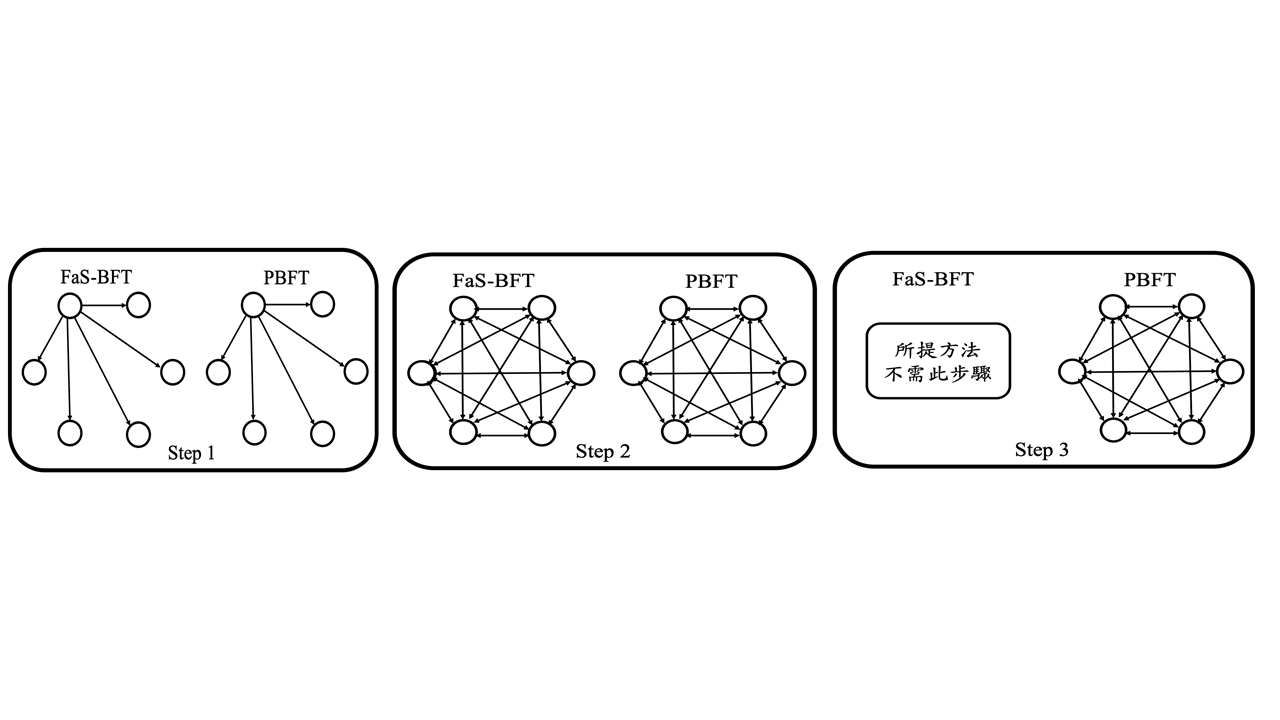
\includegraphics[scale=0.45]{images/31.png}
\caption{TwoStepBFT演算法流程圖}
\label{i:byz-latency}
\end{figure}
\subsection{Propose}\label{se_3} 
第一步:在第一個步驟中的主要目標為讓提議者廣播提議。我們稱這個廣播的訊息為Proposal訊息。 若$p$為一個Proposal訊息,則我們用$p.B$ 代表該Proposal訊息中的提議值。舉例來說,在區塊鏈中,$p.B$ 可能是該提議者產生的區塊。另外我們用$p.R$ 代表該Proposal訊息被產生的回合數。舉例來說,若$p$是第二回合的提議者廣播的Proposal訊息,則$p.R = 2$。第一步驟的虛擬碼如圖Algorithm 1 所示。我們會在解釋完第二個步驟後詳細討論第一個步驟。
\begin{algorithm}
%  \SetAlgoNoLine
  \caption{Propose:從節點$u$來觀察}
  \KwIn{節點$u$具有初始值$bin$,以及上一回合的票集合$loclset(r-1)$}
  $ldr$ = 在$r$回合的廣播提議者

  \If{$u$=$ldr$}{
   製作一個提案$p$

   $p.R$ $\gets$ $r$
   
   // 確認$p.B$並且將$p$廣播給所有節點

   \If{$r$=1}{

   $p.B$ $\gets$ $bin$ 並且將$p$廣播給所有節點

    }
  
  \ElseIf{$|loclset(r-1)|$ $\ge$ 4$f$+1}{
    
    \If{$\exists$一個$b$,且$b$$\ne$ $\varnothing$且|{$v$|$v$ $\in$$loclset(r-1)$,$v,B$=$b$ }|$\ge$ 2$f$+1}{
    $b$可以為任何值
    $p.B$ $\gets$ $b$並且將$p$廣播給所有節點
    }
    \Else{

    $p.B$ $\gets$ $bin$並且將$p$廣播給所有節點
    }

    }
    
}
   
\end{algorithm}

\subsection{Vote}\label{se_3} 
第二步:第二個步驟的主要目標為讓所有節點對接收到的Proposal訊息$p$投票,並在收到足夠多選票的情況下,提交(Commit)提議值(在區塊鏈的應用中,提交代表將區塊鏈接在區塊鏈的尾端)。為了實現這個目標,一旦節點$u$ 收到Proposal訊息$p$,則節點$u$ 首先驗證提議值$p.B$的正確性。舉例來說,在區塊鏈的應用中,節點$u$會檢查提議值$p.B$ 是否為一個合法的區塊。如果提議值$p.B$通過驗證,則$u$會廣播一個包含$p.B$ 的投票訊息(選票)。每個節點在一回合中最多只能廣播一個投票訊息。如果節點在某個預定的時間$TOcommit$內收到$4f+ 1$個投票訊息,並且這些$4f+1$的投票訊息包含相同的非空(Non-empty)提議值$b$,則節點提交提議值$b$。另一方面,如果節點$u$在時間$TOcommit$到之前無法提交,那麼節點$u$需要紀錄這個回合廣播的投票訊息中的候選值$b$,並進入下個回合。更明確地說,若$b$是在第$i$個回合中,由$u$廣播的投票訊息中的候選值,則在第$i$ + 1個回合中,如果$u$在另一個的時間$TOvote$到期之前,仍然無法收到有效的Proposal訊息,則$u$廣播的投票訊息會包含提議值$b$。值得注意的是,在第一個回合時,如果$u$ 在$TOvote$到期之前無法收到有效的Proposal訊息,則$u$ 廣播的投票訊息會包含空提議值 $\varnothing$。每當進入下一回合時,上述兩個預定時間($TOcommit$ 與$TOvote$)的長度會加倍。若 $v$ 為一個投票訊息,我們使用$p.R$和$p.B$表示$v$ 被產生的回合數和$v$中包含的提議值。第二步驟的虛擬碼如圖Algorithm 2 所示。
\begin{algorithm}
%  \SetAlgoNoLine
  \caption{Vote:從節點$u$來觀察}
    // 確認$v.B$並且將$v$廣播給所有節點



\If{在$TOvote$到期之前,$u$在第$r$回合收到一個合法的Proposal $p$}{
  $v.B$ $\gets$ $p.B$並且將$v$廣播給所有節點
}

\Else{

\If{$r$=1}{
  
  $v.B$ $\gets$ $\varnothing$
}
\Else{ 
  $v'$ $\gets$ $u$在$r$-1回合廣播的投票vote
  $v.B$ $\gets$ $v'.B$
}
    廣播$v$   
}
\If{在$TOcommit$到期之前,$u$在第$r$回合收到4$f$+1張vote訊息且包含一樣的 $b$且$b$ $\neq$ $\varnothing$}{
  
 Commit $b$

}
\Else{
進到$r$+1回合
}
  
\end{algorithm}

\subsection{Commit}\label{se_3}
Commit 階段是各節點根據上一個步驟的投票結果,判斷是否可以進行提交區塊如果存在 $lockset(h,r)$ = $b$,則提交區塊 $b$ 至區塊鏈上完成高度$h$的共識。如果 $lockset(h,r)$ = $b$不存在,則進入第一階段Propose且進入$r+1$回合。

\section{Timeout}\label{se_3}

共識中的Timeout會隨著$R$的增加進行指數型成長其成長公式為: 

$Timeout_X,_R$ = $Timeout_X$ * $TimeoutFactor^R$

其中$X$為$TOvote$或$TOcommit$,$Timeout$的起始值其值為5秒,$TimeoutFactor$預設則為2。 

\begin{figure}[!htbp]
\centering
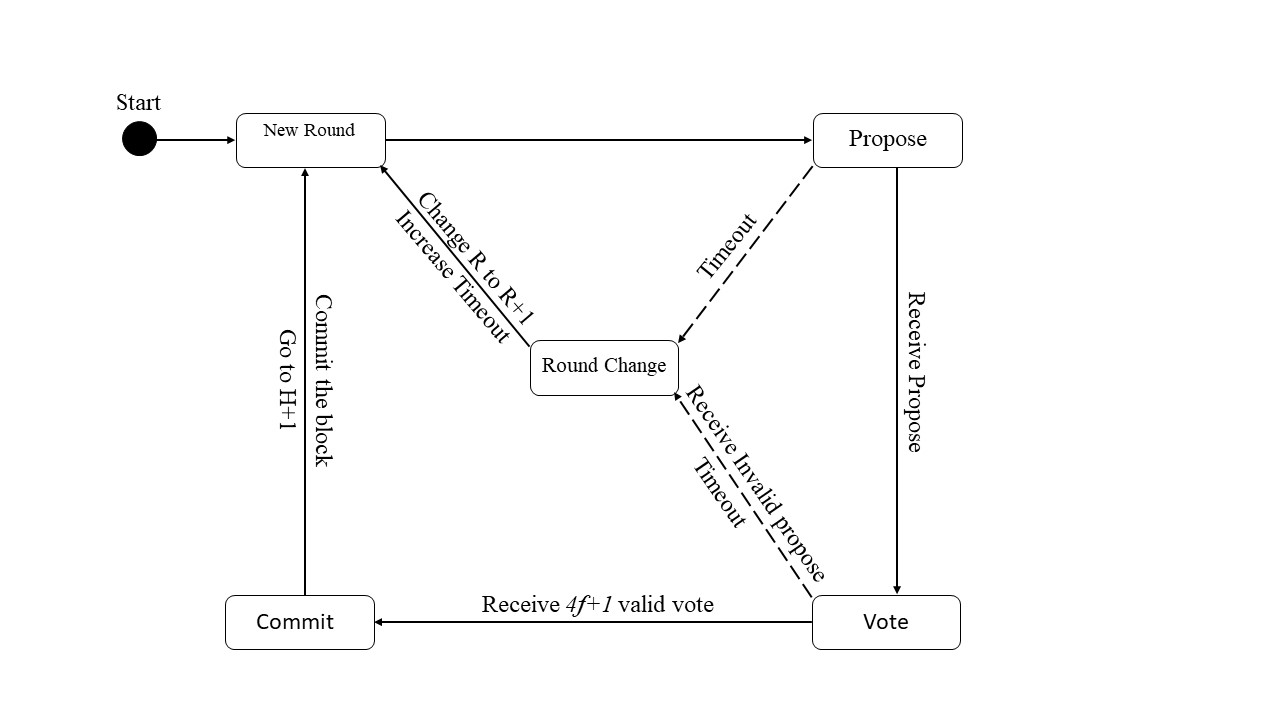
\includegraphics[scale=0.58]{images/2.jpg}
\caption{FaSBFT演算法流程圖}
\label{i:byz-latency}
\end{figure}

\chapter{安全性及活性}\label{se_4}
一個好的共識演算法必須具備安全性(SAFETY)與活性(LIVENESS),才能讓該系統保持內容一致,並且保證安全且永不出錯。
\section{安全性(SAFETY)}\label{se_4} 
共識演算法必須要確保整個網路不會有分支(Fork)產生,以確保區塊鏈的安全性。為了證明我們的演算法能夠確保安全性,我們需要證明以下兩個定理。
\begin{itemize}%项目符号开始
\item 如果兩個非故障節點$u$1和$u$2分別在同一回合$r$中提交值$b$1和$b$2,則$b$1 = $b$2。

證明:我們使用反證法,首先假設$b$1 $\ne$ $b$2,如果有一節點$u$1收到4$f$+1張提交$b$1的選票;與$u$1相同的$u$2收到4$f$+1張提交$b$2的選票。因為扣除掉可能重複投票的錯誤節點數$f$,在回合$r$裡至少有3$f$+1個非故障節點投給b1;相同的扣除掉可能重複投票的錯誤節點數$f$,在回合$r$裡至少有3$f$+1個非故障節點投給$b$2。兩個集合共6$f$+2 > 4$f$+1(非故障節點個數)。非故障節點一回合只會對一個提議投票,故矛盾。

\item 一旦有一個非錯誤的節點在$r$回合成功的提交了區塊$B$時,在未來的回合$r`$,此$r`$>$r$,只有區塊$B$能被提交。

證明:假設$Nb$是在第$r$回合中投票給$b$的節點集合。因為$b$是在回合$r$中被提交,代表|$Nb$| $\geqq$ 4$f$+1。假設$Gb$是僅包含非故障節點的$Nb$的子集。因此,|$Gb$| $\geqq$ 3$f$ +1。根據演算法規定,我們能夠觀察到如果$r$ + 1回合的廣播者擁有$r$回合的有效Lockset,那麼此Lockset必須至少包含從$Gb$發送的2$f$ + 1個投票消息。此外,對於每個候選值,假設$b$1 $\ne$ $b$2,最多只有2$f$張票在Lockset中的投票信息有包含$b$2。因此,如果下回合$r$=$r$+1的廣播者可以發送提案$p$,該$p.B$必須維持是$b$1。否則,如果$r$ + 1回合沒有Proposal,則Gb中的所有節點,仍會投票支持他們在第$r$輪投票的值,即$b$1。在這兩種情況下,$Gb$中的所有節點仍然投票對於$r$ + 1回合中的b,然後通過歸納進行Commit。
\end{itemize}

\section{活性(LIVENESS)}\label{se_4} 
我們能夠證明演算法可以保證在部分同步模型(Partially Synchronous Model)下,能夠保有的活性。

在部分同步模型的假設裡,我們假設每回合的Timeout時間都會加倍。在部分同步模型下,存在一些回合r。並且這些$r$<$r'$
所有非故障節點都可以在Timeout前接收到彼此傳來的訊息。因此,在這些$r$的下一回合$r$ + 1<$r'$回合中,如果廣播者是非故障節點
那麼廣播者必須有一個有效的lockset,並且必須有一個有效的Proposal消息。然後,所有4$f$ +1非故障節點在$r'$回合中投票給$p,B$。 由於所有這些4$f$ +1投票
消息可以及時接收,所有非故障節點都可以在循環$r'$中提交$p,B$。
\chapter{共識模組與系統架構}\label{se_5}

\section{共識模組}\label{se_5}
本章節介紹我們如何實作拜占庭容錯共識的架構。共識模組底下包含處理訊息的 Message Handler、同步訊息的 Synchronizer、與三個主要做共識的模組,Consensus Manager、Height Manager 與 Round Manager。共識模組間的關係如下圖。
\begin{figure}[h]
\centering
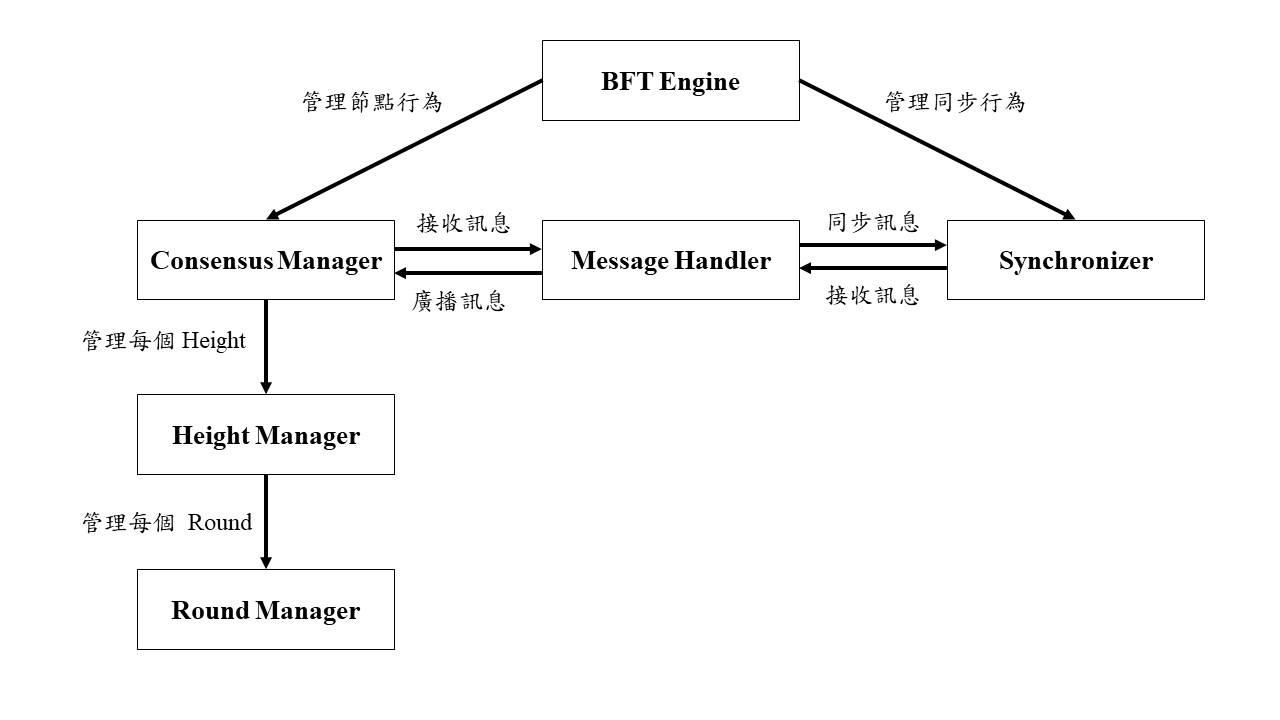
\includegraphics[scale=0.45]{images/5.jpg}
\caption{共識模組關係圖。}
\label{i:byz-latency}
\end{figure}
各共識模組之間相互負責不同事情。共識模組透過 go語言來進行實作,模組間參數時常共同管理(透過 go語言裡Channels來傳遞參數)。因此需要透過讀寫鎖,來控制讀寫流程,才不會造成多個模組同時讀寫情形。
。



\subsection{Consensus Manager}\label{se_5} 
Consensus Manager主要管理節點間連線,並且紀錄參與共識時所需的各式資訊,如:私有鏈ID、各節點地址、共識Timeout等等。
並且檢查區塊內的交易是否合法。Consensus Manager 核心技術在於定時的檢查自身狀態。如果滿足(一)廣播、(二)投票、(三)提交,任何一個狀態,則透過呼叫下層 Height Manager,進一步處理共識。同時也要將需要廣播的資訊交給 Message Handler。
\subsection{Height Manager}\label{se_5}
此模組主要功能是處理某一個高度的共識,透過管理一或多個 Round Manager 與其他節點溝通。(一)廣播:如果節點為該回合的Proposer且擁有前一回合票集合,呼叫下層 Round Manager 廣播新的共識提議;如果節點不是此回合的Proposer,等待新的共識提議被提出。(二)投票:呼叫Round Manager幫忙進行投票。(三)提交:確認高度是否已達成共識,如果還沒,則呼叫Round Manager進行提交共識。

\subsection{Round Manager}\label{se_5}
每個高度可能會需要一到多個回合,最終才能達成共識。因此Height Manager 可能須要建立多個 Round Manager 來進行共識。Round Manager 會蒐集來自 Height Manager 的訊息,經過判斷後採取對應動作。(一)廣播:對所有節點廣播共識提案、(二)投票:在一個回合裡,Round Manager只會對一個合法共識提案簽章並廣播。(三)提交:將區塊內容同步到自身資料庫,並進入下一個區塊高度。


\subsection{Message Handler}\label{se_5} 
Message handler 主要負責接收與廣播共識之中需要的訊息,在接收到來自其他節點的訊息時,進行判斷是否交給 Consensus Manager,或是過濾掉重複接受的訊息。

\subsection{Synchronizer}\label{se_5}
Synchronizer 主要目的為同步節點間訊息。因為網路間可能存在延遲,節點可能因此較晚進到共識,少了前面的訊息而無法執行共識。必須先與其他節點同步到最新狀態。  




\section{系統架構}\label{se_5}  
TwoStepBFT共識演算法相較於過去傳統三回合的共識演算法,能在網路傳輸穩定情況下,較快達成共識。我們的目標是測試TwoStepBFT在多個節點的私有鏈的效率,實驗將在AWS雲端伺服器上進行。為了達成這個目標,我們整合了許多自動化的開發套件來協助我們完成實驗。實驗系統架構主要如下圖所描述 

\begin{figure}[htbp]
\centering
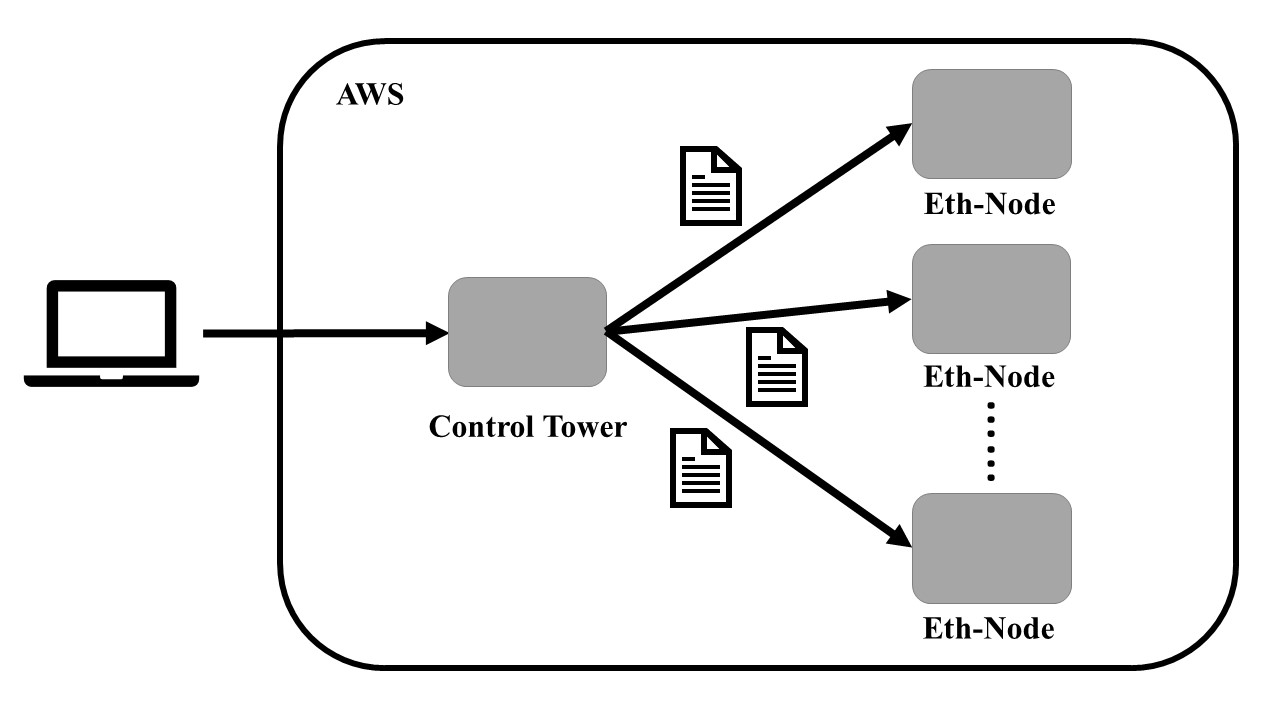
\includegraphics[scale=0.5]{images/51.jpg}
\caption{實驗系統架構圖。}
\label{i:byz-latency}
\end{figure}

該系統內含一個Control Tower,此台電腦類似實驗的中央控制中心,負責部署實驗環境到其他雲端機器上,並且收集其他機器所產生的實驗數據,該系統另包含數個區塊鏈節點,這些節點運行TwoStepBFT演算法,以達成區塊鏈共識。自動化多節點實驗主要分為兩大步驟: (1)高效率部署雲端系統 (2)自動化搭建私有鏈

\subsection{高效率部署雲端系統}\label{se_5} 
為了能夠在雲端平台上,快速開啟多台環境一致的機器,這些機器將成為區塊鏈的節點。我們整合了許多套件其中包含(一)Packer:能夠將實驗環境,打包成映像檔。這些映像黨裡會包含TwoStepBFT共識專案以及程式需要的各試工具。(二)Terraform:能夠依照使用者需求,動態產相對應的機器。
\begin{itemize}%项目符号开始
\item [1)] Packer: 為了能夠快速將上百個區塊鏈節點環境建立起來,因此使用了Hashicorp Packer這套工具來打包 AWS的AMI (Amazon Machine Images),AMI 能幫助我們快速建立出環境一致的節點。
Packer的優點如下

\item 極快速的部署:因為已經把需要的套件及其他設定都放在映像檔中,所以馬上可用。

\item 跨平台且可攜性:Packer 可針對不同平台打包出完全相同的映像檔,可在本地、雲端等各種不同平台獲得相同的運行環境。

\item 較好的測試性:映像檔一打包完成就可進行各種測試。

\item [2)] Terraform: Terraform能夠快速將AWS環境架設起來,依照使用者所撰寫程式碼搭建出所描述的架構,Terraform好處是能徹底實現基礎架構即代碼IaC (Infrastructure as code),利用代碼來配置實驗環境,讓環境安全且方便管理。
Terraform的優點如下:
\item   將基礎架構使用語法進行描述,可讓建構計劃像一般程式碼一樣進行版本控管與追蹤。 

\item Terraform會自動分析本地端計劃與遠端是否一至,自動化修改從而避免許多可能的人為操作錯誤。

\subsection{自動化搭建私有鏈}\label{se_5} 

\item [1)] Ethereum Wallet api: 系統環境建立後我們將透過Control Tower 動態產生實驗所需節點資訊,在我們的 實驗裡透過Ethereum Wallet api 動態的自動產生與實驗所需節點數之節點資訊(Public key, Address等等)

\item [2)] Genesis.json: Genesis.json 裡定義了區塊鏈資訊(包含區塊大小,區塊ID, 鏈上節點初始以太幣),由於每次實驗所產生節點帳戶地址都不相同,故我們將Genesis.json 設計成自動化動態產生,以方便實驗進行。 

\item [3)]Eth-client: 在Eth-client裡我們會執行節點間相互交易,Eth-client幫助我們每秒產生數百筆交易,鏈上的節點才能打包這些交易成為候選區塊,故與Genesis.json 相同因每次實驗所產生節點帳戶地址都不相同,我們也將Eth-client設計成自動化動態產生。 

\item [4)] Ansible: Ansible能幫助我們定義系統上的角色,方便我們依照不同角色執行相對應動作(ex. Control Tower會推送執行檔給鏈上節點執行,鏈上節點將實驗結果回傳至Control Tower做實驗分析。)

Ansible的優點如下:

\item 輕量級套件,無需在客戶端安裝agent,更新時,只需在操作機上進行一次更新即可。

\item 可將任務寫成腳本批次執行。

\item 使用python編寫,維護更簡單 。
\end{itemize}
\chapter{實驗結果} \label{se_6}
本章節對我們實作的TwoStepBFT共識版本的geth 進行測試。測試的節點皆是在Amazon EC2 t2.small上運行。t2.small 的硬體規格為1個虛擬CPU 與2GB 的記憶體。交易型態則是基本的以太坊轉帳交易。我們以交易的吞吐量Throughput(每秒共識多少筆交易量)與區塊的延遲性latency(完成一個區塊共識平均需要多少時間)與來衡量共識的效率。我們也測試共識演算法的延展性(Scalability),以瞭解當參與共識的節點數量變多時,共識效能會受到怎樣的影響。最後,我們將節點分散部屬在世界各地,讓該系統較貼近真實的應用場景。並且與同區域實驗比較。
\section{環境建設}\label{se_6}
在實驗裡所有的節點是互相連通的,即每個節點都會互相知道彼此的位置,因此我們的節點是呈現網狀連線
在佈署所有節點之後,我們先讓節點互相交易約15分鐘,讓交易存入交易池內,這讓共識時產生的區塊能夠塞滿足夠的交易。接下來將運行共識約一小時,並將結果紀錄下來。
\section{同資料中心吞吐量與延遲性測試}\label{se_6}
6.2我們將探討我們的演算法在同資料中心的實驗環境下,觀察吐量與延遲性的變化。我們將機器都運行於美國-奧勒岡資料中心。
對於測試基本的交易吞吐量與延遲性測試,我們透過控制創世區塊裡的GasLimit來控制單個區塊能包含的最大交易數量,區塊大小分別為每個區塊包含500、1000、4000、8000筆交易。實驗總共進行了五種節點數分別是16、30、60、80、100 個節點。
\begin{figure}[htp]
\centering
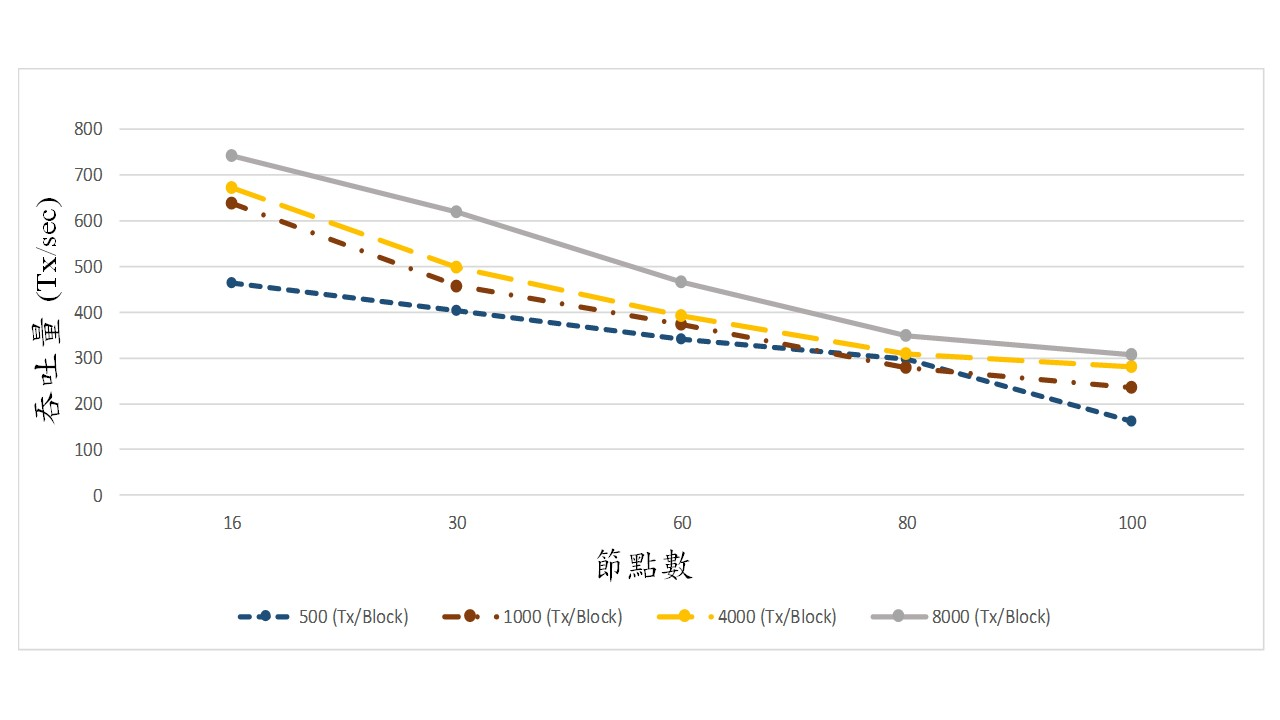
\includegraphics[scale=0.55]{images/61.png}
\caption{吞吐量 V.S 節點數}
\label{i:byz-latency}
\end{figure}
 
\newpage
\begin{figure}[h]
\centering
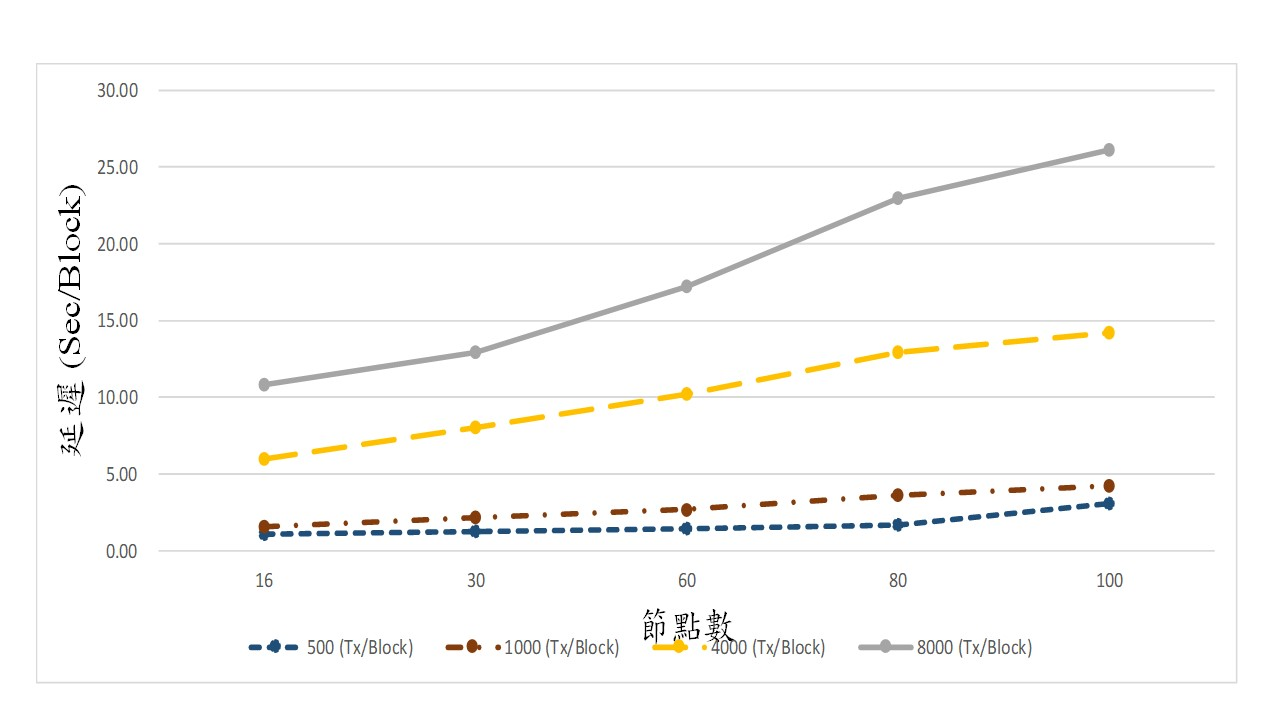
\includegraphics[scale=0.50]{images/62.jpg}
\caption{同資料中心的延遲性表現。}
\label{i:byz-latency}
\end{figure}


從圖6.1中可以看出在我們的共識演算法在節點數增加時,吞吐量隨之降低;而圖6.2則可以看出在我們的共識演算法在節點數增加時延遲也會隨之增加。當區塊大小增加時共識效率也會增加。且在100個節點吞吐量還能達到每秒300筆交易左右的共識速度,對於節點數的容忍能有良好的延展性。



\section{誇資料中心吞吐量與延遲性測試}\label{se_6}
6.3我們將探討我們的演算法在跨資料中心的實驗環境下,觀察吐量與延遲性的變化,並與同資料中心實驗進行比較。
與同區域的吞吐量與延遲性測試實驗一樣,我們先讓節點互相交易約15分鐘,讓交易存入交易池內,這讓共識時產生的區塊能夠塞滿足夠的交易。接下來將運行共識約一小時,並將結果紀錄下來。區塊大小分別為每個區塊包含500、1000、4000、8000筆交易。實驗總共進行了五種節點數分別是16、30、60、80、100 個節點。不同的是我們將節點分散的部屬在世界各地。這讓實驗更加貼近真實應用。在實驗裡我們將節點平均分散在(美國-奧勒岡、美國-維吉尼亞北部、日本-東京、新加玻、倫敦)
\begin{figure}[htp]
\centering
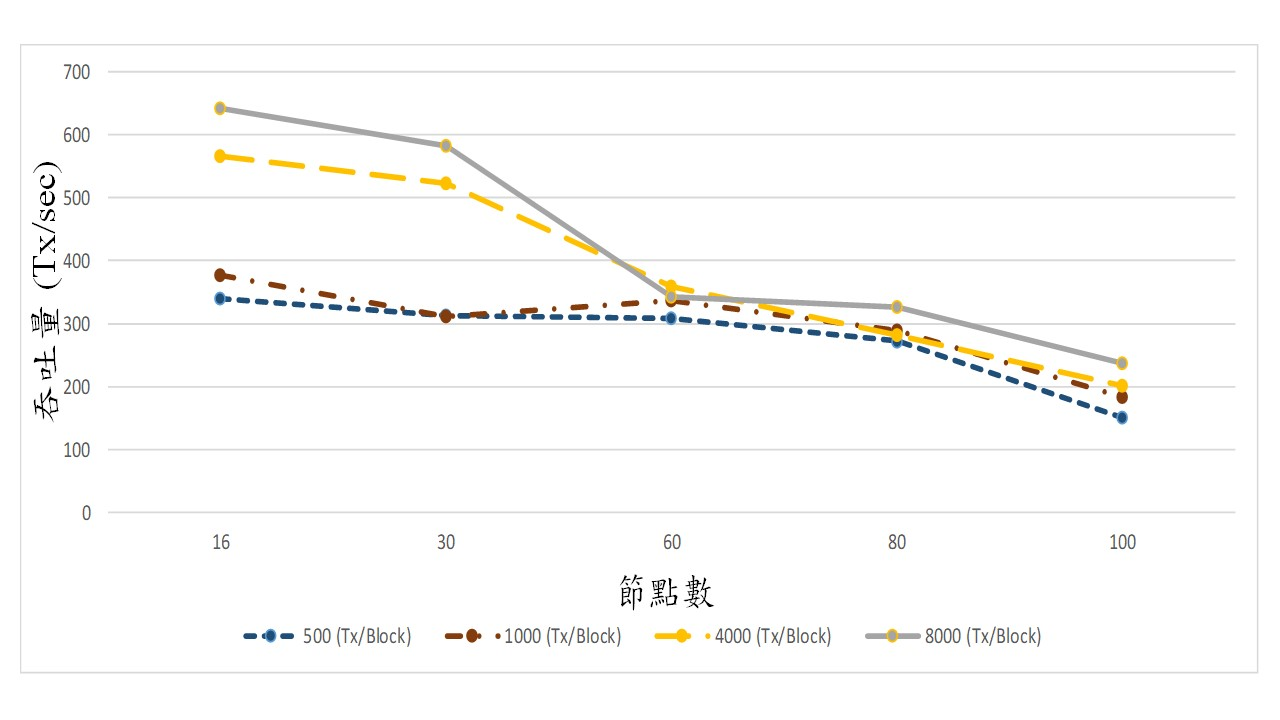
\includegraphics[scale=0.5]{images/63.jpg}
\caption{跨資料中心的交易吞吐量表現。}
\label{i:byz-latency}
\end{figure}

\begin{figure}[htp]
\centering
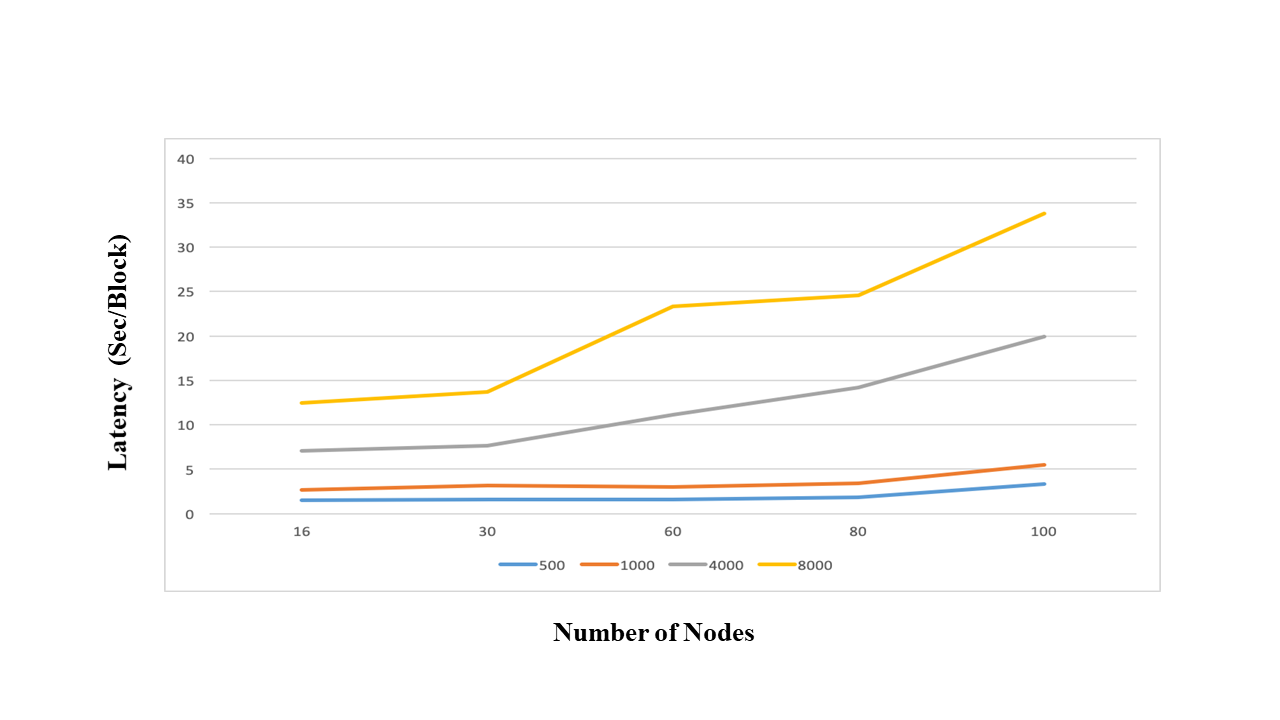
\includegraphics[scale=0.5]{images/64.jpg}
\caption{跨資料中心的延遲性表現。}
\label{i:byz-latency}
\end{figure}


在同區域的實驗裡,結果顯示在區塊大小為1000以上(Tx/Block)時,實驗結果穩定;但在區塊大小翻倍情況下,吞吐量並無大幅上升,但4000與8000的延遲卻大幅上升。也就是說在不同區域驗裡1000(Tx/Block)是一個較穩定的結果。從圖中也能觀察到在不同區域的實驗裡,吞吐量幾乎皆小於同區域的實驗,延遲也較同區域的實驗高。但即使在不同區域裡,100個節點的共識吞吐量也維持約有300TPS左右。

\begin{figure}[htp]
\centering
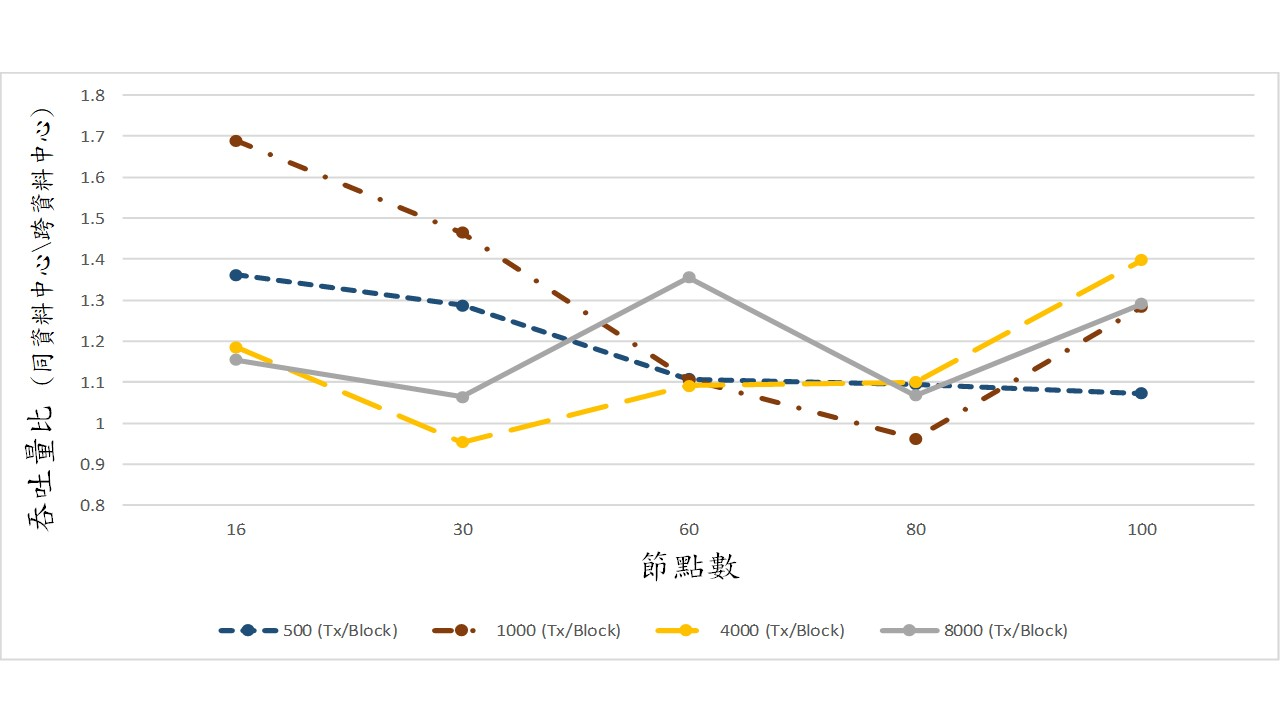
\includegraphics[scale=0.5]{images/65.jpg}
\caption{同資料中心與跨資料中心吞吐量比。}
\label{i:byz-latency}
\end{figure}

\begin{figure}[h]
\centering
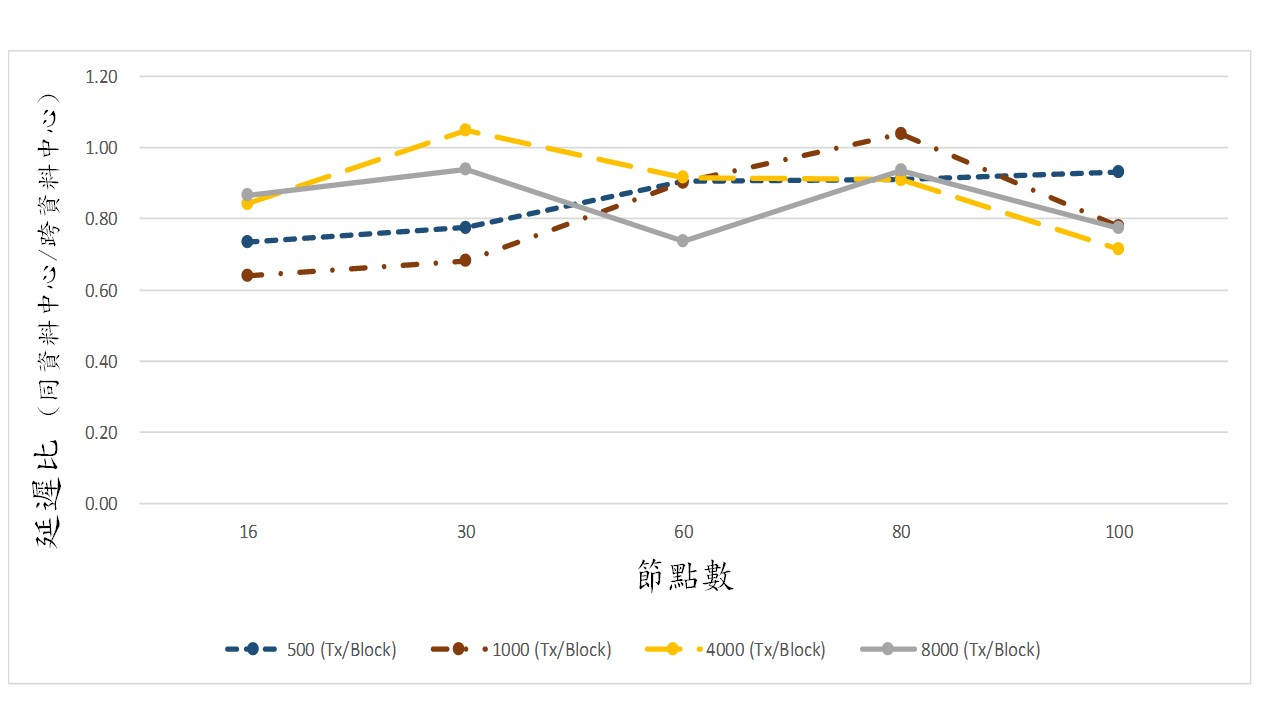
\includegraphics[scale=0.8]{images/66.jpg}
\caption{同資料中心與跨資料中心延遲比。}
\label{i:byz-latency}
\end{figure}



\chapter{相關研究}\label{se_7}
\section{公有鏈上共識演算法}\label{se_7}
\subsection{Proof-of-Work}\label{se_7} 
比特幣是目前最著名的區塊鏈應用,使用PoW(Proof-of-Work)作為比特幣的共識系統。在該系統裡節點需要花費時間與電腦運算資源,嘗試解出一組數學公式的答案,用來獲得廣播區塊的權力。該答案也稱之為Nonce。將Nonce值附於區塊內,其他節點就能透過簡單數學公式,驗證該答案是否有效。除非能控制超過51\%以上的系統運算能力,才能進行攻擊。在私有鏈上因為參與共識的節點較少,因此系統內計算能力總和非常小。攻擊者可以輕易地以較高的計算能力,推翻過去的共識結果,因此私有鏈不傾向選擇使用PoW。
著名的以太坊\cite{Ethereum}也是使用PoW作為共識機制。以太坊除了能夠儲存交易外,還能執行程式碼,運行智能合約。
\subsection{Proof-of-Stack}\label{se_7}
PoS(Proof-of-Stack)是把持有資產數量作為參考。資產數量越多者,越有機會擔任下個區塊的廣播者。PoS認為持有資產量高的人會越傾向維護貨幣價值,因此發動攻擊的可能性越低。不過PoS缺點也非常明顯,PoS很可能造成貨幣不流通。如果貨幣不流通,該貨幣也失去其價值。PPCoin\cite{vasin2014blackcoin}是目前少數運行PoS的區塊鏈。
\subsection{混合型共識演算法}\label{se_7}
混合型共識演算法概念是從公有鏈節點中,隨機挑選一群人運行拜占庭容錯共識演算法。這類的方法需要具有非常公平的抽籤演算法。Algorand\cite{gilad2017algorand}作為一個混合型共識演算法,最重要的一個機制便是引入了VRF(Verifiable Random Function),中文稱作可驗證隨機函數。透過該函數,區塊鏈上節點能夠自行驗證是否成為該回合的提議者,並且能夠提出證明供其他節點進行驗證。Algorand的處理能力超過1000TPS且延遲低於五秒。


\section{私有鏈上共識演算法}\label{se_7}
\subsection{Proof-of-Authority}\label{se_7}
PoS(Proof-of-Authority)是由一群授權的節點來負責驗證區塊與廣播區塊。不同於PoW驗證節點不需強大的運算能力,也不需要像PoS得擁有很多資產才能廣播區塊。但此節點必須是大家公認的已知節點,且通過一定程度身分驗證。一旦節點勾結其他節點進行攻擊,那鏈上的其他管理者可以移除或替換這些惡意節點。目前以太坊在原始碼中也提供PoA共識演算法名為Clique共識演算法。

\subsection{三步驟拜占庭共識演算法}\label{se_7}

BFT是拜占庭容錯(Byzantine-Fault-Tolerant)的縮寫。在拜占庭容錯的私有區塊鏈上,即使系統中部分節點當機或存在惡意節點情況下,區塊鏈依舊具備安全性(Safety)與活性(Liveness)等性質。一般來說,一個回合需要執行三個步驟。第一個步驟為播其提議;第二個步驟透過交互投票,檢查該提議者是否只有廣播一份提議;第三個步驟節點便開始投票,若一個節點蒐集到足夠多的同意票,便可以確認共識結果。知名的BFT演算法PBFT\cite{castro1999practical}便是根據上述三個步驟設計。而許多私有鏈區外鏈系統,都是根據上述想法而延伸出來。例如:Tendermint[3] 是一種區塊鏈共識機制主要以 Go 語言撰寫,與 PBFT 相似,每個回合都是一次廣播與兩次投票來產生共識,不同於 PBFT 之處在於Tendermint 引入 Lock 概念,藉此維護系統的 Safety 和 Liveness。在官方文件裡提及理想狀況下 64 個節點能有約 4000 TPS。MSIG­-BFT 是一個三步驟的共識演算法,與一般BFT演算法不同的是透過收集 f +1 個數位簽章來確保共識提議唯一性,讓共識演算法保證安全性及唯一性。目前MSIG­-BFT 實做在 go­-ethereum上。LibraBFT\cite{STEVE_HANNA2010}是 Libra 區塊鏈系統所使用的共識系統,在 LibraBFT 技術白皮書提到,選擇 Hotstuff\cite{yin2018hotstuff} 作為 LibraBFT 的演算法基礎。Hotstuff 採用了聚集簽名,讓系統內的訊息傳輸量從 $O(n^2)$ 變成 $O(n)$,在 libra 白皮書裡提到,理想狀況下 100 個節點仍有約 1000 TPS。

\subsection{兩步驟拜占庭共識演算法}\label{se_7}
過去也有少部分的BFT演算法在一個回合中只需要兩個步驟,例子包含FaB\cite{abraham2018revisiting}、Zyzzyva\cite{kotla2007zyzzyva}、SBFT\cite{martin2006fast}、Hydrachain\cite{Hydrachain}。然而,FaB與Zyzzyva已被指出無法保證活性,換句話說,共識演算法可能永遠無法達成共識。另一方面,Hydrachain也被指出無法保證安全性,也就是說,不同的正常節點可能會有不同的共識節果,這在區塊鏈上及代表分岔。雖然SBFT能夠保證安全性與活性,但是在有拜占庭攻擊時,會改用類似PBFT的三步驟設計。因此,在系統狀況良好時,SBFT每回合只需要執行兩個步驟。但是在系統狀況不良時,SBFT每回合仍需要執行三個步驟。在 100 個節點情況下吞吐量約50 TPS。



\chapter{討論與結論}\label{se_8}
\section{討論}\label{se_8} 
下面我們探討影響共識效率可能因素如:

\begin{itemize}%项目符号开始

\item 節點數影響共識效率 :
節點數量上升會導致傳輸時間拉長,所以完成每個步驟時間都與節點數有關。在演算法設計裡,初始Timeout長度是固定的,如果初始的Timeout設定過低且未考慮傳輸時間,演算法會頻繁的Timeout更換新回合。進而拖慢整體共識效率。

\item 區塊大小影響共識效率:
從實驗裡發現隨著區塊大小變大,共識吞吐量也會隨之增加,但增長幅度有限會趨於平緩;然而共識延遲雖也會隨之增加,但增長幅度卻急遽上升。
因此,我們推斷隨著區塊大小變大,吞吐量將隨之增加,但會趨於平緩甚至下降。然而延遲卻會不斷上升且越來越急遽。因此,我們無法透過無限制增加區塊大小,來增加我們共識效率。


\end{itemize}

\section{結論}\label{se_8}
TwoStepBFT是一種新的兩步驟拜占庭共識演算法,可以保證部分同步假設下的安全性和活躍性。該演算法在任何情況下都只需要兩個步驟,不須額外複雜的方法來達成共識。通過實驗結果,我們知道共識吞吐量與延遲都與節點數息息相關。在AWS 上測試TwoStepBFT效率皆能達到數百TPS。並且透過將節點分散搭建在世界各地,讓實驗更加符合真實應用場景,且吞吐量依舊能維持約300 TPS。

透過學習其他共識演算法,TwoStepBFT未來也能持續改進,例如:(1)Hotstuff透過聚集簽名,來降低系統傳輸複雜度。(2)由於BFT類的演算法透過輪流廣播訊息來達成共識,如果共識期間存在錯誤節點將會拖慢整體共識效率,因此如果能將錯誤節點排出共識系統,將能增加安全性並且提高共識效率。



\@startappendix



\backmatter

\clearpages
\phantomsection
\addcontentsline{toc}{chapter}{\bibname}
\bibliographystyle{abbrv}


% Your bibliography goes here

\bibliography{thesis}
\end{document}
